\section{Kommunikation mellem drone og server}

Dette afsnit beskriver testen af kommunikationen mellem drone og server. 

Kommunikationen er testet ved at bruge 3G modulet på drone som benytter HTTP protokollens med GET og PUT metoder. 
Idet serveren er en passiv enhed, er det 3G modulet der skal tage initiativet til at hente eller sende data. 

På figur \ref{fig:integrationstest_webserver} vises hvordan informationen på serveren ser ud. Ved et GET, ønskes disse information hentet ned. 

\begin{figure}[H]
\centering
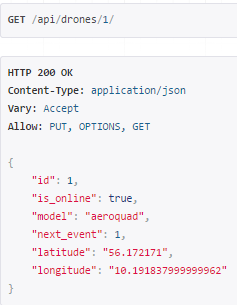
\includegraphics[width=0.4\textwidth]{Billeder/Test/integratest_webserver.png}
\caption{Webserver UI}
\label{fig:integrationstest_webserver}
\end{figure}

Ved brug af GET metoden på serverens URL (iha-11726.iha.dk/api/drones/1/), får 3G modulet informationen på figur \ref{fig:getfromserver} returneret. Dette information deles op i en header og body, hvor headeren kasseres og body sorteres ved hjælp af et JSon bibliotek.

\begin{figure}[H]
\centering
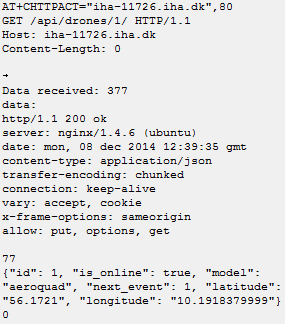
\includegraphics[width=0.4\textwidth]{Billeder/Test/getfromserver.png}
\caption{GET data fra server}
\label{fig:getfromserver}
\end{figure}